\documentclass[11pt,xcolor=svgnames]{beamer}
\usepackage{dsfont,natbib,setspace,changepage,multirow}
\mode<presentation>

% replaces beamer foot with simple page number
\setbeamertemplate{navigation symbols}{}
\setbeamercolor{frametitle}{fg=black}
\setbeamerfont{frametitle}{series=\bfseries}
\setbeamerfont{frametitle}{size=\normalsize}
\newcommand{\theme}{\color{Maroon}}

\setbeamertemplate{footline}{
   \raisebox{5pt}{\makebox[\paperwidth]{\hfill\makebox[20pt]{\color{gray}\scriptsize\insertframenumber}}}}

\graphicspath{{../graphs/}}

% colors
\newcommand{\bk}{\color{black}}
\newcommand{\rd}{\color{red}}
\newcommand{\fg}{\color{ForestGreen}}
\newcommand{\bl}{\color{blue}} 
\newcommand{\gr}{\color{gray}}
\newcommand{\sg}{\color{DarkSlateGray}}
\newcommand{\nv}{\color{Navy}}
\setbeamercolor{itemize item}{fg=gray}

% common math markups
\newcommand{\bs}[1]{\boldsymbol{#1}}
\newcommand{\mc}[1]{\mathcal{#1}}
\newcommand{\mr}[1]{\mathrm{#1}}
\newcommand{\bm}[1]{\mathbf{#1}}
\newcommand{\ds}[1]{\mathds{#1}}
\newcommand{\indep}{\perp\!\!\!\perp}

% spacing and style shorthand
\setstretch{1.1}

% shorthand
\newcommand{\sk}{\vspace{.5cm}}
\newcommand{\R}[1]{{\tt \nv #1}}
\newcommand{\til}{{\footnotesize$\bs{\stackrel{\sim}{}}$ }}
\DeclareSymbolFont{extraup}{U}{zavm}{m}{n}
\DeclareMathSymbol{\vardiamond}{\mathalpha}{extraup}{87}

\begin{document}

\setcounter{page}{0}
{ \usebackgroundtemplate{
\includegraphics[height=\paperheight]{phoenix}}
\begin{frame}[plain]
\begin{center}

{\bf \Large [1] Big Data: Inference at Scale}


\vskip 1.5cm 
Matt Taddy, University of Chicago Booth School of Business

\vskip .2cm 
\texttt{faculty.chicagobooth.edu/matt.taddy/teaching} 


\end{center}
\end{frame} }


\begin{frame}
{[1] \theme  getting oriented}

\begin{adjustwidth}{.25in}{}
Introduction: \sg goals, material, syllabus\bk

\sk
Computing 
\begin{itemize} 
\item  {\bk R:} examples, resources, and how we'll learn.
\item  Big data, distribution, storage, connectivity.
\end{itemize}

\sk
Visualization, Statistics, and Dimension Reduction

\sk
Testing and Discovery: \sg False Discovery Rates

\end{adjustwidth}

\end{frame}

\begin{frame}
{Introduction}

{\bf This is a class about \theme Inference at Scale}
\sk

We're here to make sure you have the tools for making \\good decisions based on large and complicated data.

\sk A mix of practice and principles
\begin{itemize}
\item Solid understanding of essential statistical principles.
\item Concrete analysis ability and best-practice guidelines.
\end{itemize}

\sk
We'll learn what to trust, how to use it, {\it and how to learn more}.


\sk {\nv A hands-on subject:} the idea that MBAs can just pass data analysis off to number crunchers is an out-of-date cartoon.  

\end{frame}



\begin{frame}

{\bf 
{\theme What is in a name?} \\Big Data, Econometrics, Statistics, and Machine Learning }


\sk
There are many labels for what we do...

\vskip .2cm
Econometrics $\rightarrow$ Statistics \\ \hskip .5cm $\rightarrow$ Data Mining /  Big Data / Data Science  \\ \hfill $\rightarrow$ Machine Learning (ML) and Artificial Intelligence (AI)

\vskip .5cm
Along this spectrum, you move from heavy focus on what things you are measuring (what real phenomena they correspond to) to a more pragmatic `useful is true' pattern discovery approach.
\vskip .25cm
The similarities are much bigger than any distinctions.

\end{frame}

\begin{frame}


The `{\theme BD}' name  comes from computer scientists working to do aggregation on data that is too big to fit on a single machine.


\vskip .1cm
As aggregation became analysis, BD got closer to stats + ML. 

And after a healthy dose of hype, everything is fairly confused...

\sk
My take: {\it Data Science} is the umbrella term for inference in a world that is messier that in your old statistic textbook, and {\it Big Data} is DS focused on business and industrial applications.

\begin{itemize}
\item Infer patterns from complex  high dimensional data.
\item Simplicity and scaleability of algorithms is essential.
\item We keep an eye on both {\it useful} and {\it true}.
\item The end product is a {\it decision}.
\end{itemize}


\end{frame}


\begin{frame}

A big aspect of Big Data is `pattern discovery' or `{\theme data mining}'

\sk
Economists think data mining is a dirty word ...

\begin{center}\bk \vskip -.25cm

{\gr Economics and the  Lucas Critique}

\vskip .2cm
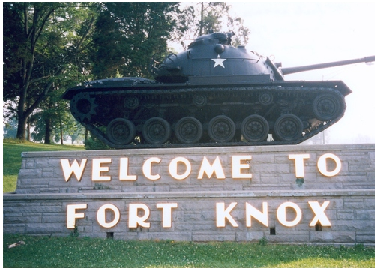
\includegraphics[width=2.2in]{../graphs/FortKnox}
\end{center}

\bk
{ \hfill ... but they only know {\theme bad} data mining.}

\end{frame}


\begin{frame}

{\bf Good DM is about inferring useful signal at massive scale.}

\vskip .75cm
Our goal is to summarize really high dimensional data in such a way
that you can relate it to { structural models} of interest.
\\
\vskip .2cm\hfill{\bk $\Rightarrow$ Variable Selection and Dimension Reduction}

\vskip .75cm
{ We also want to predict!} If things don't change too much...
\\
\vskip .2cm\hfill { \bk $\Rightarrow$ Probabilistic Prediction and
  Classification Rules}

\bk \vskip .75cm
{\bf \hfill We need to constantly beware of {\theme false discovery}.}

\end{frame}


\begin{frame}

{\bf 
What does it mean to be `big'?}

\sk
Big in  both  the number of observations ({\theme size `n'})\\
and in the number of variables ({\theme dimension `p'}).

\sk In these settings, you {\theme cannot}:

{\small \sg
\vskip .01cm
Look at each individual variable and make a decision ({\it t-tests}).

\vskip .01cm
Choose amongst a small set of candidate models ({\it F-test}).

\vskip .01cm
Plot every variable to look for interactions or transformations.\\
}

\sk
Some BD tools are straight out of previous statistics classes
({\theme linear regression}) and some are totally new ({\theme
  trees, PCA}).\\
{\gr All require a different approach when {\it n} and {\it p}
  get really big.}

\end{frame}



\begin{frame}

{\bf Course Schedule}

\sk {\gr subject to change... }

\vskip .1cm
\begin{itemize}\small
\item[{[1]}] {\theme Data:} Computing, plotting, and
  principles.  [False?] discovery.
\item[{[2]}] {\theme Regression:} A grand overview, linear and
  logistic.
\item[{[3]}] {\theme Model Selection:} penalties, information criteria,
cross-validation
\item[{[4]}] {\theme Treatment Effects:} HD controls, propensity scores, bootstrap
\item[{[5]}] {\theme Classification:} Multinomials,  KNN, sensitivity/specificity, DMR
\item[]{\bf Midterm!}
\item[{[6]}] {\theme Networks:} co-occurance, directed graphs, Page Rank
\item[{[7]}] {\theme Clustering:} Mixture models, k-means, and association rules.  
\item[{[8]}] {\theme Factors:} Latent variables, PCA, PCR, and
  PLS.
\item[{[9]}]{\theme Trees:} CART and random forests, ensembles
\item[{[10]}]{\theme Text Mining:} topic models, sentiment prediction, deep learning
\end{itemize}

\end{frame}

\begin{frame}

{\bf We'll be working with  real data analysis examples}

\vskip .25cm
\begin{itemize}
\item Mining client information: {\gr Who buys your stuff,
    what do they pay, what do they think of your new product?}
\item Online behavior tracking: {\gr Who is on what websites,
    what do they buy, how do/can we affect behavior?}
\item Collaborative filtering: {\gr predict preferences from
    people who do what you do; space-time recommender engines. }
\item Text mining: {\gr Connect blogs/emails/news to sentiment, beliefs, or intent. Parsing unstructured data, e.g. EMR.}
\item Big covariates: {\gr mining data to predict asset prices; using unstructured data as controls in observational studies}. 
\end{itemize}

\sk
Many are applicable to marketing, but we're far more general.

\end{frame}



\begin{frame}

{\bf All of our analysis will be conducted in \theme R} 

\sk
This is the real deal: industrial 
strength software for data analysis. It's free, cross
platform,  and hugely capable.

\sk 
Academics {\gr(stats, marketing/finance, genetics, engineering)}, \\ companies
{\gr(EBay, Google, Microsoft, Boeing, Citadel, IBM)}, and  governments
{\gr (Rand, DOE National Labs, Navy) } {\theme use R}.

\sk{
Since R is free, you'll always be able to use it.}

\end{frame}


\begin{frame}

{A huge strength of R is that it is open-source.}\\
{This is also why it is sometimes a bit unpolished.}

\sk
R has a {\nv core}, to which you can add contributed {\nv
  packages}.
{These add-ons are as varied as the people who write them.}
Some are specific, others general, some are great, some suck.

\sk
R is not without flaws, but neither are the other options.\\
{\gr e.g., I like python, but the community of stats developers is smaller and you need to be a more careful programmer. }


\sk 
Some students prefer to wrap R in an IDE; e.g. R-studio.
\end{frame}


\begin{frame}

The barrier of entry for R is its  command line  interface:

{\nv \hfill You type commands to get what you want.~~~~~~~~~~~~~~}

\sk
The learning curve can be steep, but is very worthwhile.
\begin{itemize}
\item You have code of saved commands, so you know what
  you've done and can easily repeat similar operations.
\item {\theme Interacting with computers in this way is a Big Data skill.}
\end{itemize}

\sk
All code for lectures and homework will be available
online.  \\{ The best way to learn software is through imitation. }

\sk There are a ton of resources: see the website and {\bf syllabus}.

\end{frame}


%%%%%%%%%%%%%%%%%%%%%%%%%%%%%%
%% break for syllabus here %%%
%%%%%%%%%%%%%%%%%%%%%%%%%%%%%%

\begin{frame}
{Computing: \theme R}



To start,  click on 
\includegraphics[width=.25in]{Rlogo}~ or ~
\includegraphics[width=.3in]{rstudio} ~{\gr or just type `R' in a terminal.}


\vskip .25cm
At its most basic, R's just a fancy calculator.
(e.g., \R{*,/,+,-}).


\vskip .25cm
Everything is based on assigning names \\{\gr (\R{\gr<-} works pretty much the same as \R{\gr=})}.
\begin{itemize}
\item[] \R{A <- 2} $\rightarrow$ \R{\rd 2}.
\item[] \R{B <- c(1,2,3)} $\rightarrow$ \R{\rd 1  2  3} (same as
  \R{B=1:3}).
\item[] \R{C = A + B[3]} $\rightarrow$ \R{\rd 5}.
\end{itemize}

\vskip .25cm
The \R{c(~)} function and \R{:} operator build {\theme vectors}.\\
{\tt length(B)} will tell you how many elements it holds (3). \\

\vskip .25cm
To inspect a variable, just type the name ({\theme do this often!}).

\end{frame}


\begin{frame}

{\bf R can read almost any data format}

\sk
First, set the {\theme working directory} to where you store
data.

{\gr It's good practice to create folders just for
  this.}

{Use \R{cmd-D}  (Mac), \R{File $\!\!\rightarrow\!\!$ ChangeDir} (Windows)\\ or  just type \R{setwd(`/path/to/my/working/dir')}.}  \\
{\gr Set a default with {\it preferences} or shortcut
{\it properties}.}


\sk
In this directory, you'll store {\theme flat files}: text tables of data.

We'll use mostly {\tt\theme .csv} files: comma separated values.

{\gr Any file in Excel can be saved as `.csv', and
vice versa. 

Beware of of Excel automatically changing data values!}

\vskip .25cm
~~~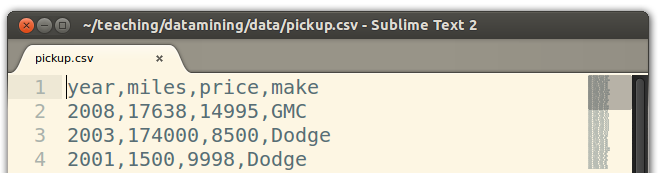
\includegraphics[width=4in]{csvfiletop}
\vskip -1cm
\end{frame}


\begin{frame}[fragile]

{To load data, type \R{trucks <- read.csv("pickup.csv")}.}

The data are then in {\theme working memory} (RAM).


\sk

\R{trucks} is a \R{dataframe}: a matrix with names.  

You can use index names and numbers to access the data.

{\small \nv
\begin{semiverbatim}
trucks[1,] {\bk# the first observation}
trucks[1:10,] {\bk# the first 10 observations}
trucks[,1] {\bk# the first variable (year)}
trucks\$year {\bk# same thing}
trucks[,'year'] {\bk# same thing again}
trucks[trucks\$miles>200000,] {\bk# some real clunkers}
\end{semiverbatim}}

And call R's functions on the data.
{\small \nv
\begin{semiverbatim}
nrow(trucks) {\bk# sample size}
summary(trucks) {\bk# summary of each variable}
\end{semiverbatim}}

\vskip -.5cm
\end{frame}



\begin{frame}
{A note on \theme data storage}


\vskip .25cm
{\gr Much of the world revolves around flat files (.txt, .csv, etc).

There are two other dominant broad storage/analysis modes.}


\sk
{\bf Structured Query Language (SQL) databases}  

\vskip .25cm
A model for fast relational
  queries on structured data: 

\vskip .1cm
~~{\small \bk select \sg apple\_id,apple\_price \bk from \sg grocerylist
  \bk where
  \sg apple\_col = green}

\vskip .1cm
{\gr Examples are MySQL, Oracle, SQLite, Teradata, ...}


\vskip .25cm
The analyst typically pulls data from the DB with an SQL query, writes this to a flat file, then reads the flat file into R.

\vskip .1cm
Packages like RSQLite can also read directly from SQL DBs.

\vskip .1cm
{\it After} extraction, you analyze the data {\it in memory}.

\end{frame}

\begin{frame}

{\bf Distributed File Systems (DFS)}  
\vskip -1cm
\hskip 6cm 
\includegraphics[width=.6in]{../graphs/hadoop_logo}

\includegraphics[width=.9in]{../graphs/spark}\hspace{.2in}


When the data is unstructured (log files, raw text documents)\\
or too big to fit on a single server, we turn to DFS models.
\vskip .1cm
{\gr Examples are Hadoop HDFS, Amazon S3.}

\vskip .1cm  The data is scattered across many machines, \\with a key that tells you where all the pieces live.

\vskip .25cm  
Analysis uses algorithm frameworks like MapReduce:\\
partition data into small chunks, analyze each independently.

\vskip .25cm  

{\theme\bf This is Big Data}

\vskip .1cm  
{\gr
Each chunk analysis (`reduce') uses the sort of tools we'll cover in class. We'll talk more about distributed algorithms later, and throughout class we always focus on scalable techniques.}

\end{frame}


\begin{frame}
{Back to R}

{\bf Basic Elements in R: \theme numeric, factor, logical, character}

\sk
The values in our dataframes all have a {\theme class}.
\begin{itemize}
\item {\theme numeric} values are just numbers {\gr (1, 2, 0.56, 10.2)}.
\item {\theme factor} variables are categories with {\theme levels} {\gr(`lowfat',`reg')}
\item {\theme logical} values are either {\theme TRUE} or {\theme
    FALSE}.
\item {\theme character} strings are just words or messages
  {\gr(`hi mom')}.
\end{itemize}

\sk
We have plenty of tools to investigate and manipulate these:

\vskip .1cm
\R{as.numeric(X), factor(X), class(X), levels(X)}
\end{frame}


\begin{frame}

{\bf R has functions that look like \R{f(arg1, arg2, ...)}.}

~e.g., create new variables: \R{ lprice = log(trucks\$price)}.

~And add them to your data: \R{truck\$lprice = lprice}. 

To find out how a function works, type \R{?f} or \R{help(f)}.

\vskip .75cm
{\bf Plotting \bk is super intuitive}

\begin{itemize} \bk
\item[]  Use \R{plot(mydata\$X, lY)} or
\R{plot(lY \til  mydata\$X) }
\end{itemize}
{Let's look at some basic plots...}

\end{frame}

\begin{frame}

{\bf The simple {\theme histogram} for continuous variables}

\vskip .3cm
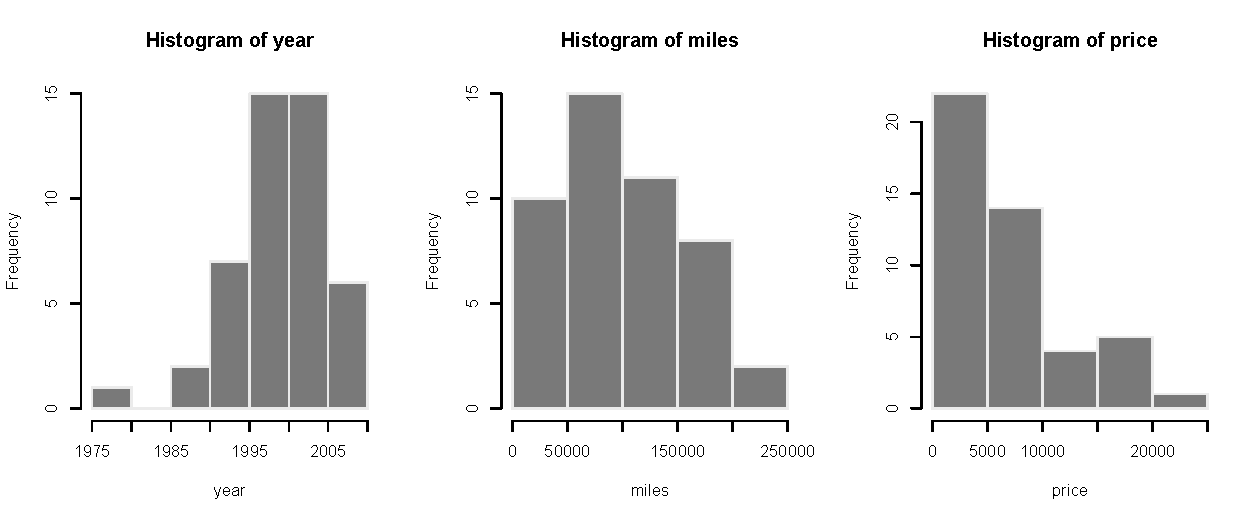
\includegraphics[width=4.3in]{../graphs/puhist}

\small \sg
Data is {\theme binned} and plotted bar height is the count in each bin.
\end{frame}



\begin{frame}

{\bf {\theme Boxplots:} summarizing conditional distributions }

\vskip -.75cm
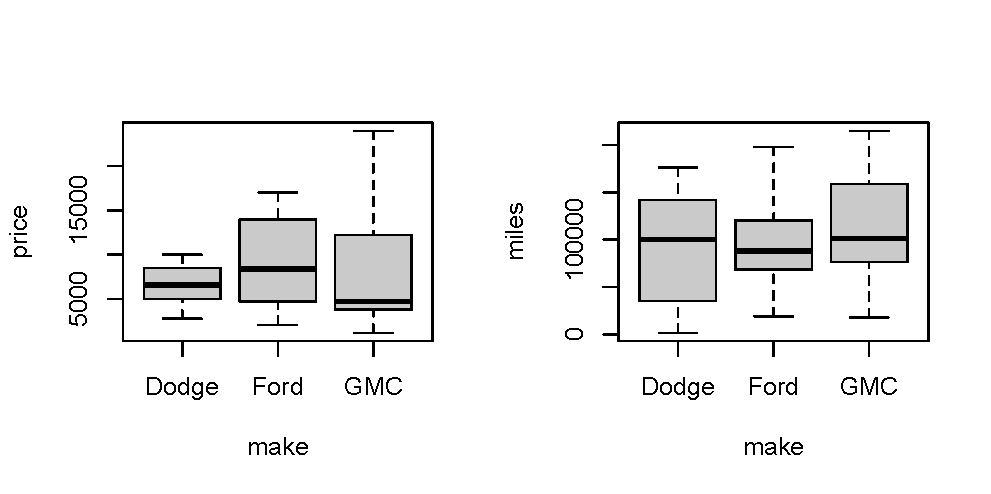
\includegraphics[width=4.4in]{../graphs/carsType} \vskip -.2cm
\footnotesize \sg
The box is the {\theme Interquartile Range} (IQR; i.e.,
$25^{th}$ to $75^{th}$ \%), with the median in bold.  The {\theme
  whiskers}
extend to the most extreme point which is no more than 1.5 times
the IQR width from the box.

\end{frame}

\begin{frame}

{\bf Use \theme scatterplots \bk to compare variables.\vskip .3cm }

\vskip -.8cm
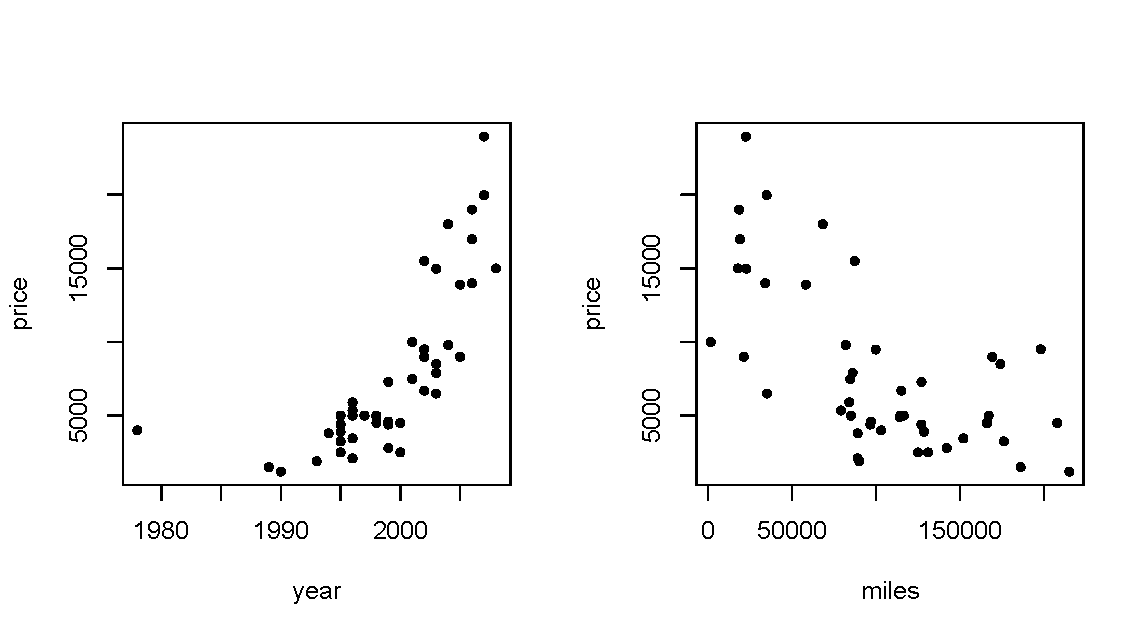
\includegraphics[width=4.3in]{../graphs/puscatter}

\end{frame}

\begin{frame}

{\bf And \theme color \bk them to see another dimension.}\vskip .3cm

\vskip -.8cm
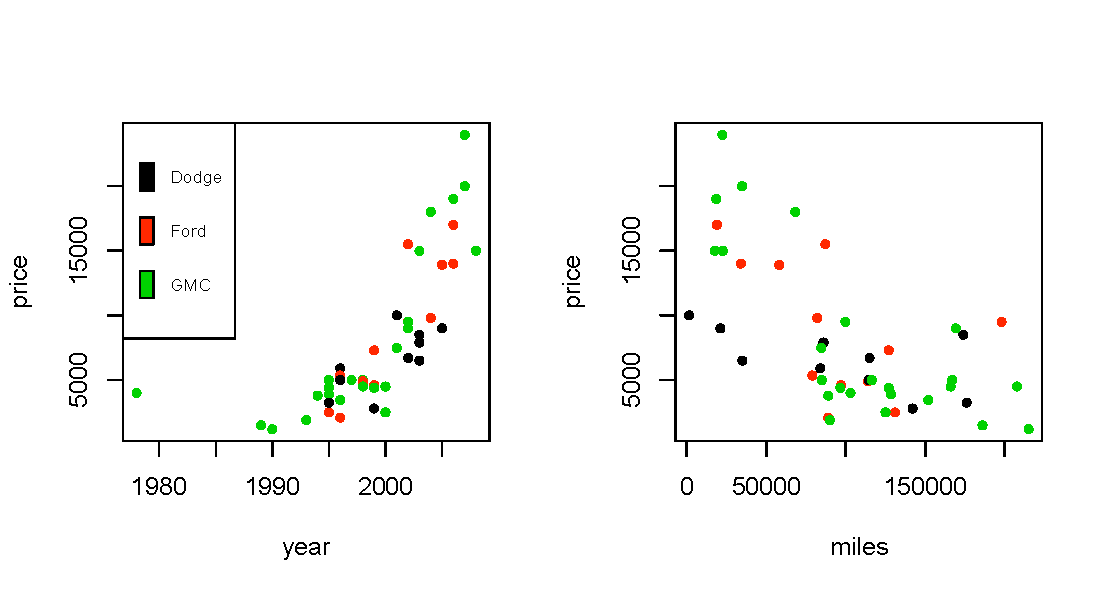
\includegraphics[width=4.4in]{../graphs/puscattercol}

\sg The scatterplot is mightier than you think...
\end{frame}


\begin{frame}

{\bf Scatterplots are a fundamental unit of statistics.}\\

\sk If you're able to find and compare meaningful low-dimensional
summary statistics, then you are {\theme winning} the DM game.
\begin{itemize}
\item Humans are good at comparing a few variables.
\item If we can put it in a picture, we can build intuition.
\item Prediction is easy in low dimensions.
\end{itemize}
 
\sk
The key to good graphics is to
reduce high-dimensional data to a few very
 informative  summary statistics, then plot them.\\
{\gr We'll focus on info visualization throughout this course.}

\end{frame}


\begin{frame}
{A note on \theme data visualization}

A plot without a concept of a variable is useless
graphic. 

\vskip .5cm
Three broad pillars:
\begin{itemize}
\item {\nv Statistics:} reducing dimension of your data to a few rich variables for comparison.
{\gr Can be just picking two features to scatterplot, or can involve more complicated projections.}
\item {\nv Design:} effective communication -- with shapes, space, and color -- for a given set of variable observations.
\item {\nv Language:} making it easy to move from Stats to Design.
\end{itemize}

\vskip .25cm
They're all interconnected, but we'll focus on statistics.  

\end{frame}

\begin{frame}

{\bf Fancy plot: \bk monthly stock returns}

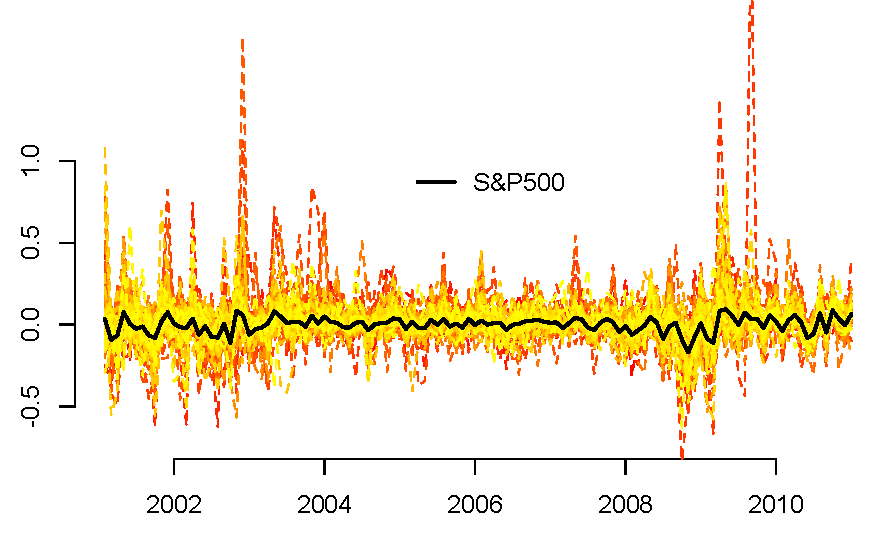
\includegraphics[width=4.25in]{fancyret}

\vskip .25cm
\hfill{\nv What do we learn?}

\vskip -.5cm
\end{frame}



\begin{frame}

{\bf Useful plot: \bk market model coefficients}

\vskip .25cm
Fit a line between stock returns $R_t$ and market returns $M_t$ (SP).
\[
R_t \approx \alpha + \beta M_t
\]
$\alpha$ is money you make regardless of what the market does.\\
$\beta$ is the asset's sensitivity to broad market movements.

\begin{center}
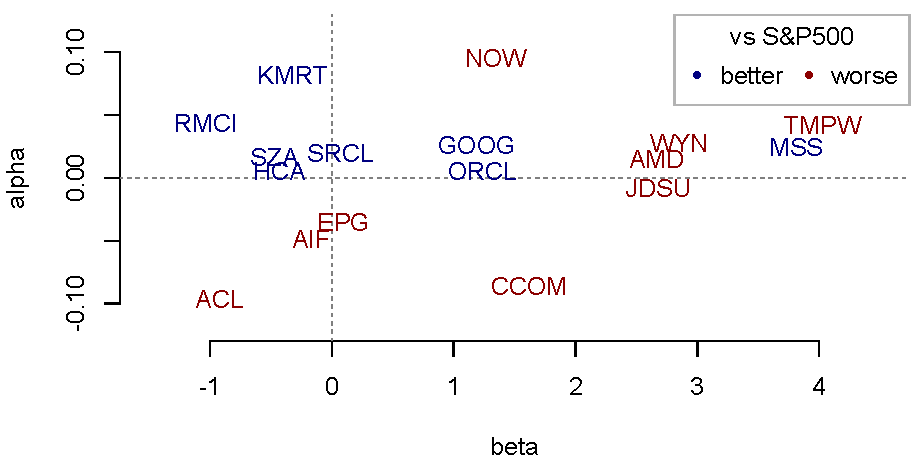
\includegraphics[width=3.5in]{usefulret}
\end{center}
\vskip -1cm
\end{frame}


%%%%%%%%%%%%%%%%%%%%%%%%
%%% another break here %
%%%%%%%%%%%%%%%%%%%%%%%%


\begin{frame}[fragile]
{Regression is king}

{\small \nv
\begin{semiverbatim}
fit <- glm(log(price)\til{year+make}, data=trucks)
summary(fit) {\gr # glm = generalized linear model}
...\bk
Coefficients:
              Estimate Std. Error t value Pr(>|t|)    
(Intercept) -195.22731   25.18120  -7.753 1.24e-09 ***
year           0.10196    0.01259   8.099 4.07e-10 ***
makeFord       0.13987    0.19786   0.707    0.484    
makeGMC        0.16202    0.17586   0.921    0.362    
\end{semiverbatim}}

This is the model {\gr (familiarize yourself with the notation!)}
\[
\ds{E}[\log({\tt price})] = \beta_0 + {\tt year}\beta_{\tt year} + 
\ds{1}_{[\tt ford]}\beta_{\tt ford} +  \ds{1}_{[\tt gmc]}\beta_{\tt gmc}.
\]
See other models and syntax in {\tt pickups.R}.  

We'll see more next week: review the basics before then.

\end{frame}

\begin{frame}
{Review: \theme Hypothesis Testing}


What is \R{Pr(>|t|)}?  Why the \R{***}?


\sk
For a test of $\beta=0$ vs $\beta\neq 0$, the test stat is  
$z_\beta = \hat{\beta}/s_{\hat{\beta}}$:

\vskip .1cm how many standard deviations is our estimate away from zero? 

\vskip .1cm
The {\theme p-value} is then 
$\theme \mr{P}( |Z| > |z_{\hat{\beta}} |)$, with $Z \sim \mr{N}(0,1)$.

\sk
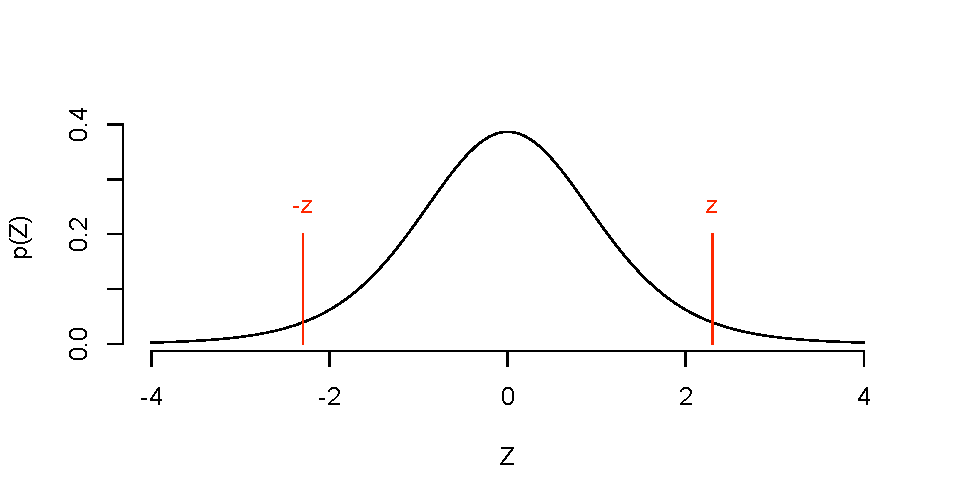
\includegraphics[width=4.25in]{../graphs/plevel}\\
\vskip -.5cm

\end{frame}

\begin{frame}

{\bf A single test}

\sk
{A p-value is  probability of a test
stat farther into the distribution tail than what you've observed, {\it if the null hypothesis is true}.}

\sk
{\nv Testing procedure:}
Choose a cut-off `$\theme \alpha$' for your p-value `$\theme p$', and conclude
significance (e.g., variable association) for {\theme$p<\alpha$}.

\sk
This is justified as giving only $\alpha$ probability of a 
  false-positive.
{\sg  For example, in regression, 
$\hat\beta \neq 0$ only if its $p$-value is less than the accepted
risk of a false discovery for each coefficient.}

\end{frame}

% \begin{frame}
% {Review: \theme Contingency Tables}

% Discovering association / testing independence via\\
% factor on factor
% comparisons in a { contingency table}

% \begin{center}\small\bk
% \begin{tabular}{l c c}
% &\multicolumn{2}{c}{\sc Belief in an Afterlife} \\
% \sc Gender \hspace{1cm} & Yes \hspace{1cm}
% & No/Unsure \\
% \hline
% Females & 509 \hspace{1cm} &116\\
% Males & 398 \hspace{1cm} & 104 \\
% \hline
% \end{tabular}

% \vskip .2cm
% \scriptsize \gr \it \hskip -3cm NORC: 1998 General Social Survey
% \end{center}

% \hfill This tabulates {\theme cross-classification} of two factors.

% \sk
% If two factors are independent, then
% any level of one should have the same probability for
% each level of the other factor.

% \end{frame}


% \begin{frame}

% {\bf Pearson chi-squared tests for independence }

% \sk
% Consider a table with $i=1...\mr{I}$ rows and $j=1...\mr{J}$ columns.

% \vskip .25cm
% {\nv  If the two factors are independent}, 
% expected cell counts are 
% $E_{ij} = \text{row.total}_i\times\text{column.total}_j/N$.
% and
%  the
% statistic
% \[
% Z = \sum_i \sum_j \frac{ (N_{ij} - E_{ij})^2 }{E_{ij}}
% \]
% has $\chi^2$ distribution with $df = (I\!-\!1)(J\!-\!1)$ degrees of
% freedom.

% \sk
% {\gr The continuity approximation that requires $E_{ij}
%   \geq 5$ish.   Some software make small changes, but
% this is the basic formula. }

% \end{frame}





% \begin{frame}

% {\bf \nv Independence of Sex and the Afterlife }

% {\footnotesize
% \[
% \theme z \gr = \frac{(509-503)^2}{503} + \frac{(398-404)^2}{404} +
% \frac{(116-122)^2}{122} + \frac{(104-98)^2}{98}  \theme \approx 0.8
% \]}

% 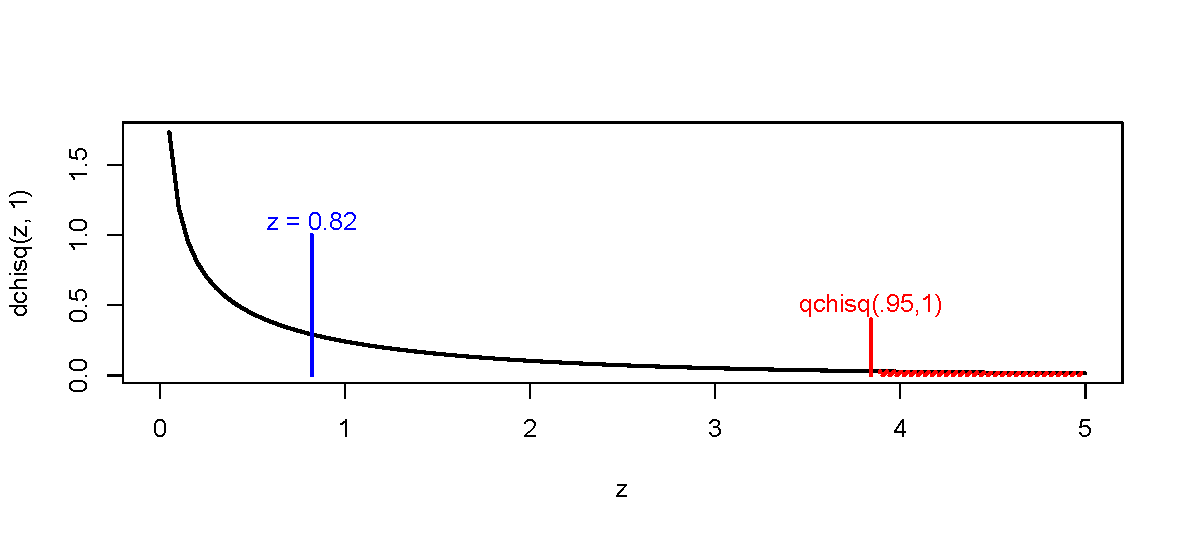
\includegraphics[width=4.5in]{chi2b}

%  No association between gender and afterlife
% beliefs.


% \end{frame}


\begin{frame}

{\bf The problem of multiplicity}

\vskip .25cm
$\alpha$ is for a single test.  If you repeat many tests, 
about $\alpha\times$100\% of the null tests 
should erroneously pop up as significant.



\sk 
{
Suppose that 5  of  100 regression coefficients are actually
influential, and that you  find all of them significant.

\vskip .1cm
Test the rest of them at $\alpha=0.05$:

\vskip .1cm 
~~Since you reject $H_0$ for 5\% of the useless 95 variables, \\
~~{\nv $4.75/9.75  \approx$ 50\% of significant tests are
false discoveries!} }

\sk 
This is called the False Discovery Proportion (FDP).

It can be really big with a small true non-Null rate.

\end{frame}


\begin{frame}
{False Discovery Rate}

\sk
Big data is about making {\it many} tough decisions.

\vskip .05cm

Instead of focusing on single tests, we'll consider 

\sk
~~~~~~~~~~~$\displaystyle
\text{FD~Proportion} = \frac{\mr{\#~false~positives}}{\mr{\#~tests~called~significant}}
$

\sk
FDP is a property of our fitted model.  We can't know it.

\vskip .25cm

But we can control its expectation:

\vskip .1cm
~~~~~~~~~~~{\theme False Discovery Rate, 
FDR $= \ds{E}[\text{FDP}]$}.



\vskip .1cm
It is the multivariate (aggregate) analogue of $\alpha$.


\end{frame}

\begin{frame}

{\bf False Discovery Rate control} 

\sk
Suppose we want to be sure that FDR $\leq$ $q$ (say, 0.1). 

\sk
{\nv The Benjamini {\tt+} Hochberg (BH) algorithm:}

\vskip .25cm
$\bullet$ Rank your $N$ p-values, smallest to largest, $p_{(1)} \ldots
p_{(N)}$.

\vskip .15cm

$\bullet$ Set the p-value cut-off as $p^{\star} = \max\left\{p_{(k)} : p_{(k)} \leq
  q\frac{k}{N}\right\}$.

\sk
{If your rejection region is p-values $\leq p^\star$, then $\text{FDR} \leq
  q$.}


{\gr Caution: assumes (rough) independence between tests.}

\end{frame}


\begin{frame}

{\bf $\vardiamond$ \nv Motivating FDR control}

\sk
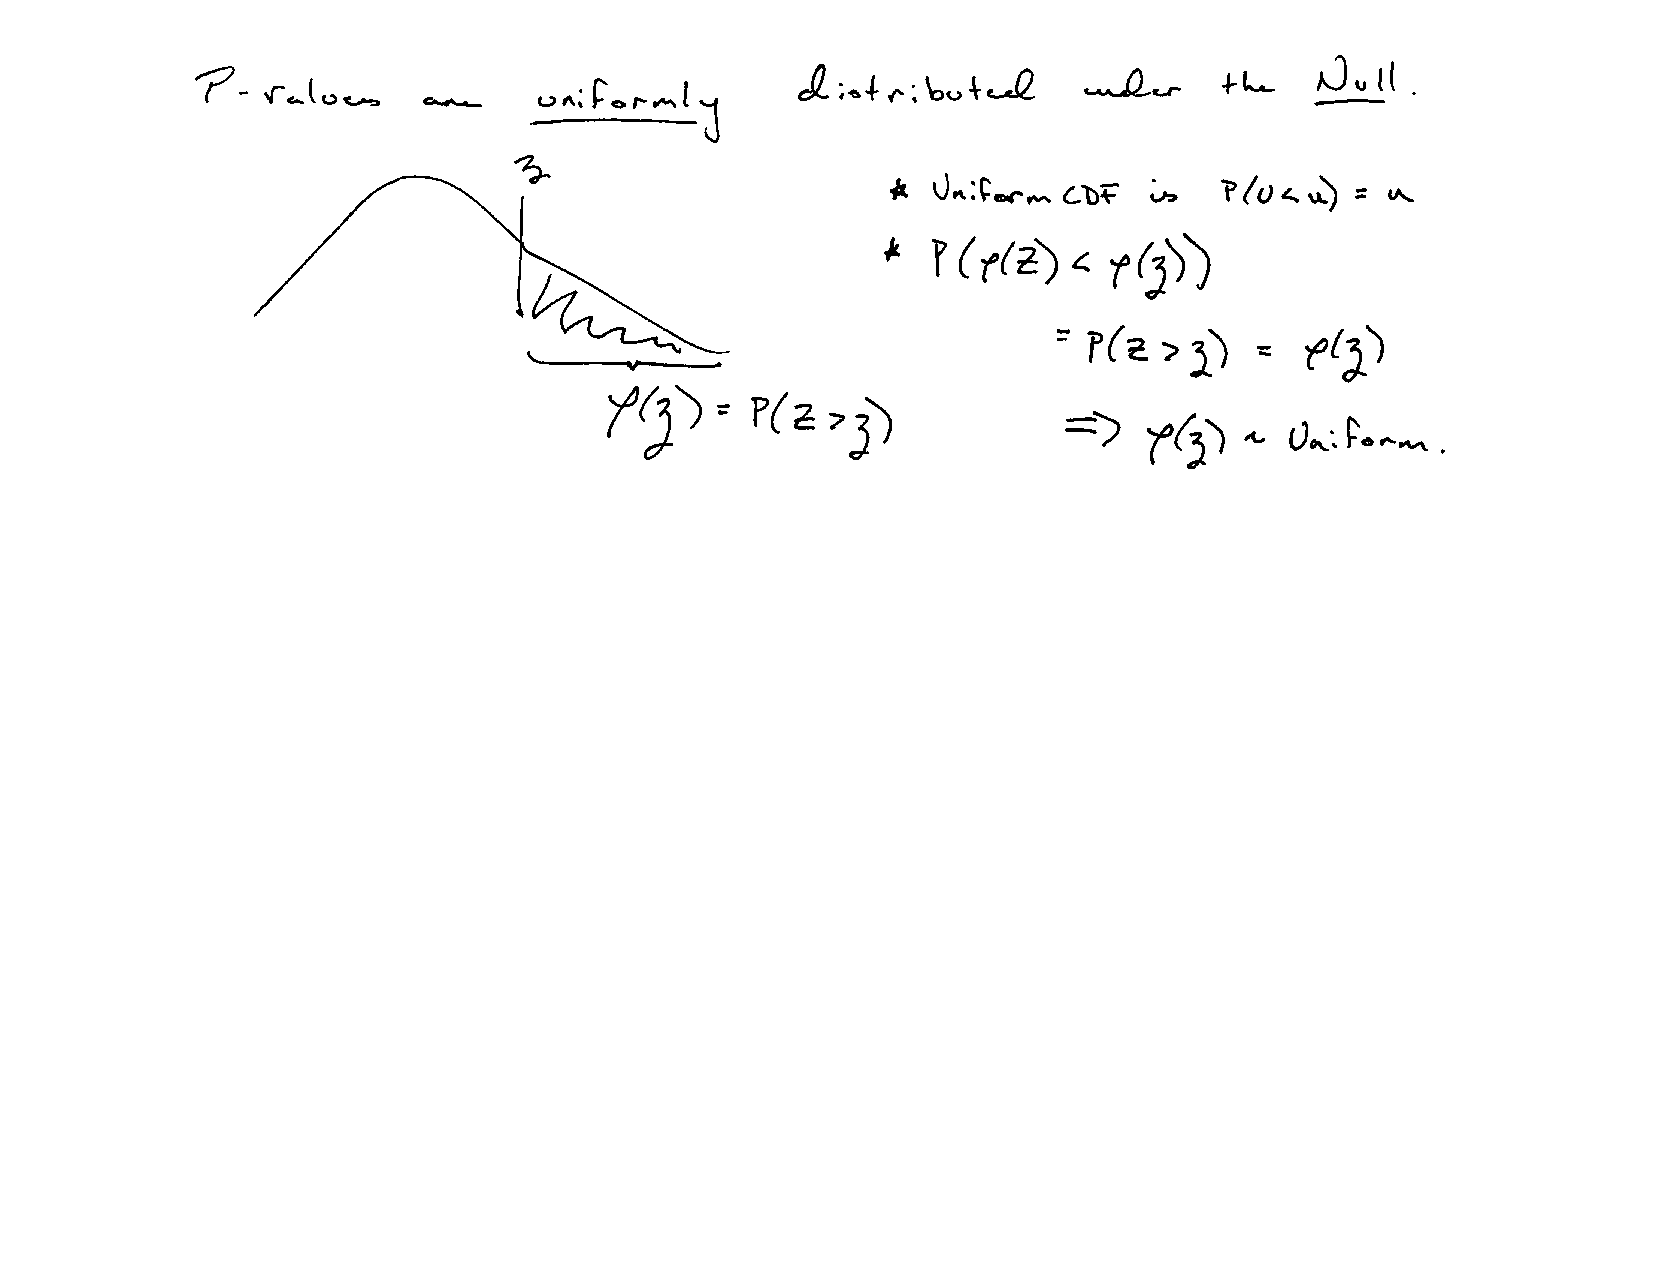
\includegraphics[width=4.25in]{pvalpit}\\
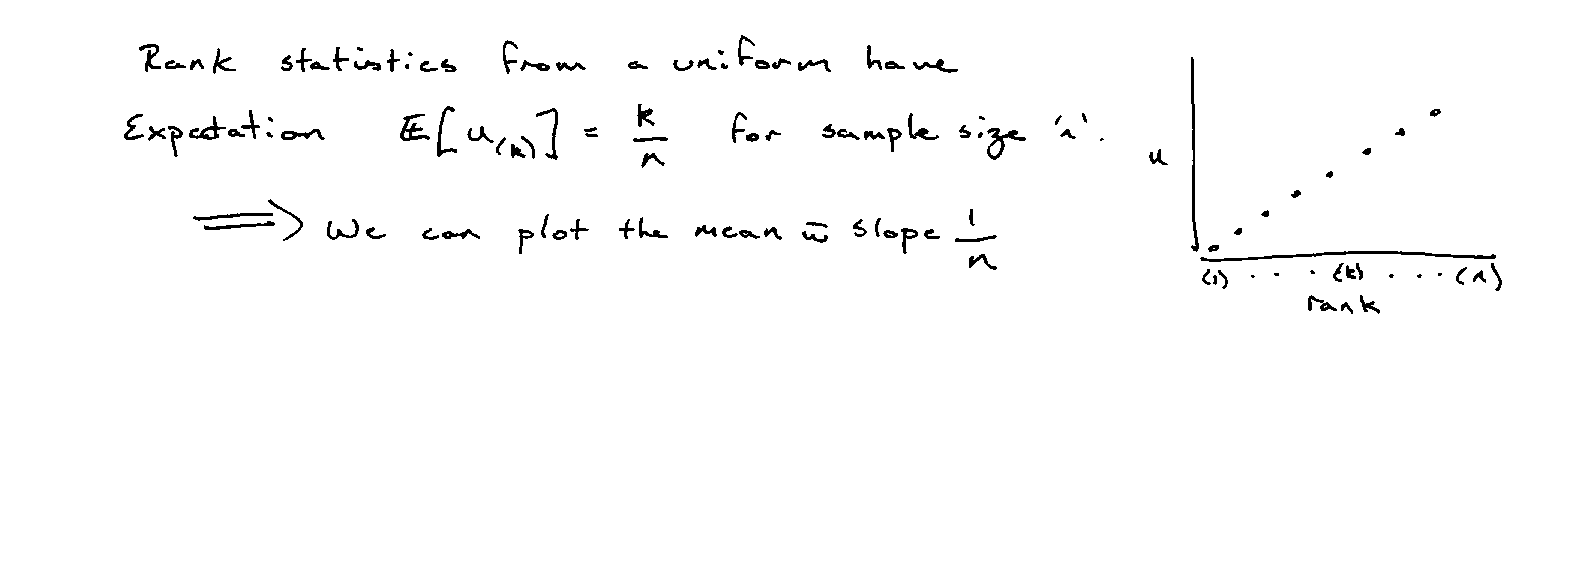
\includegraphics[width=4.25in]{pvalrank}


\vskip .2cm
{\gr $\theme q$ is the slope of a shallower line defining our rejection region.}


\end{frame}


\begin{frame}

{$\vardiamond\vardiamond$ \nv \bf  Demonstrating FDR control}

\vskip .25cm
Given our independence assumption the proof is simple.

\vskip .25cm
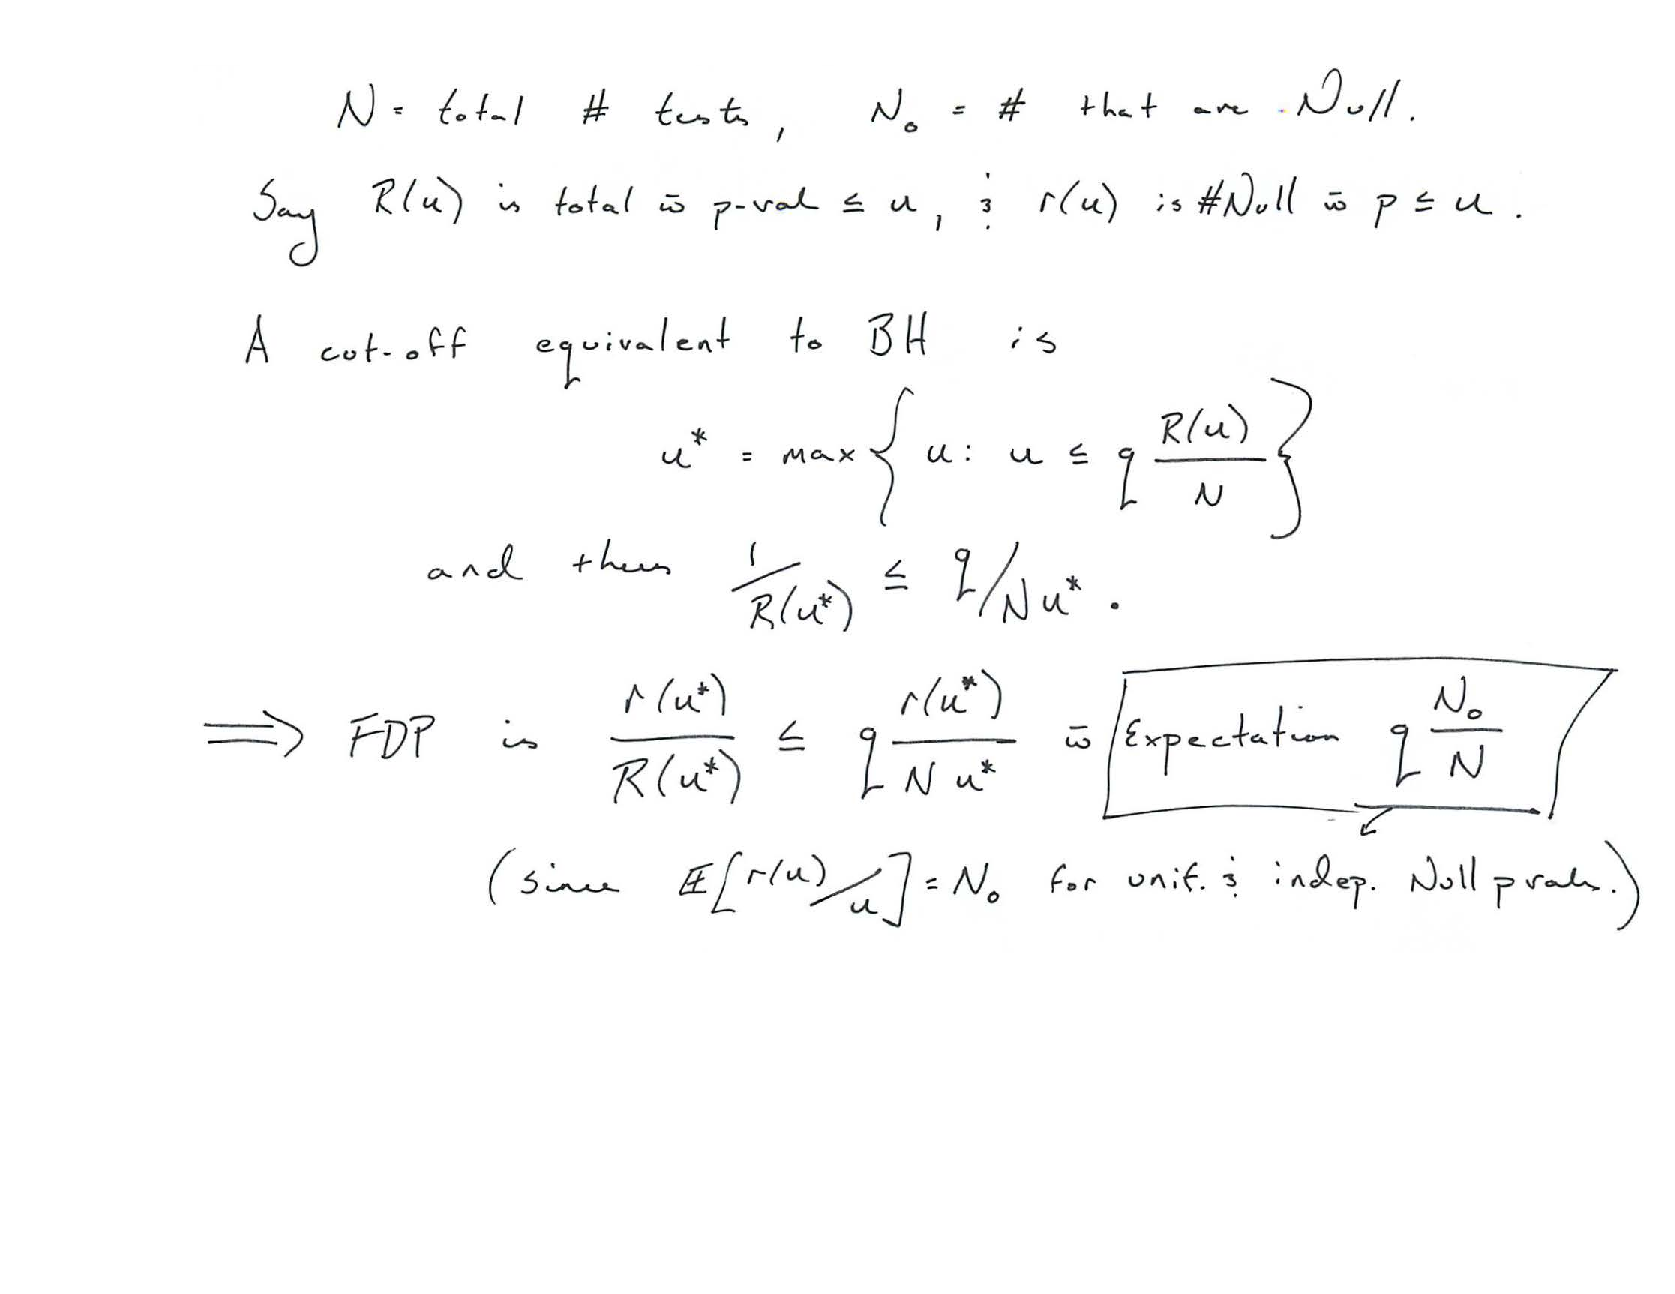
\includegraphics[width=4.25in]{fdrproof}\\


\end{frame}

\begin{frame}

{\bf \theme FDR roundup}

\sk
We introduced the problem of {\it multiplicity} by saying that given $\alpha$ (p-value cutoffs) can lead to big FDR: $\nv \alpha \rightarrow q(\alpha)$

\sk
B+H reverse the relationship -- it's a recipe for the $\alpha(q)$ that will give you whatever FDR $q$ you want: $\nv q \rightarrow \alpha(q)$

\sk
FDR is {\it the} way to summarize risk when you have many tests.\\
You'll never think about testing the same again!

\end{frame}

\begin{frame}
{\theme Example: \bk multiple testing in GWAS}


{\it GWAS: genome-wide association studies}

Scan large DNA sequences for association with disease.\\

\sk
Single-nucleotide polymorphisms (SNPs) are paired DNA locations that
vary across chromosomes.  The allele that occurs most often is
  major ({\theme A}), and the other is minor ({\theme a}).

\sk
\nv Question: \bk Which variants are associated with increased
risk? \\
\hfill{\gr Then investigate why + how.}

\vskip .5cm
\hspace{-.45in} 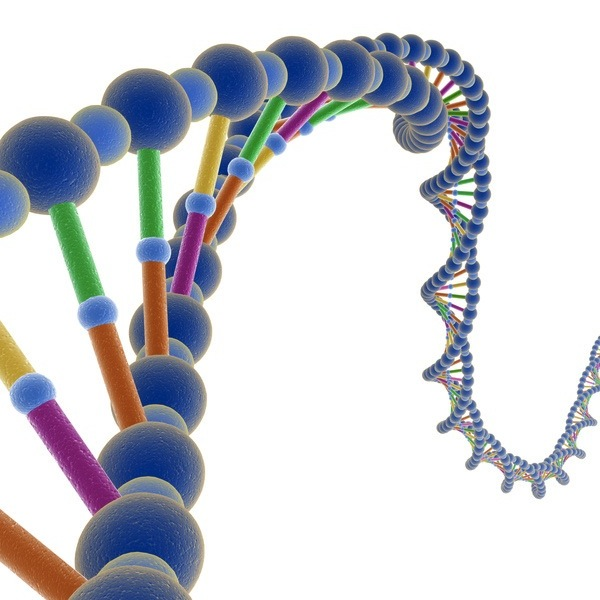
\includegraphics[width=3.5in,height=1in]{dna}
\vspace{-.8in}


\end{frame}


\begin{frame}

{\bf \bk Allele Association}

\sk A common SNP summary is Allele Frequency (AF):

\vskip .2cm
\hfill {\nv freq(a):}~~~{\theme
{AA $\rightarrow$ 0} ~~~~ {Aa/aA $\rightarrow$ 1} ~~~~ {aa $\rightarrow$ 2} ~~~~~~~~~~~~}

\vskip .2cm Question:  {\sg which SNP AF distributions that vary with
disease?}

\vskip .1cm
 Answer: {\sg a huge number of AF$\times$disease contingency tables.}

\sk
An example for type-2 Diabetes mellitus:

\bk
\begin{center}\small
\begin{tabular}{l c c c}
&\multicolumn{3}{c}{minor AF: {\footnotesize \tt rs6577581} } \\
\sc dm2 status \hspace{1cm} & 0~
& 1 & 2 \\
\hline
case & 357 ~& 72 & 27 \\
control & 428  ~& 54 & 1 \\
\hline
\end{tabular}

\vskip .2cm
\it $\chi^2$ stat is 32 on 2 $df$ for $p=9${\scriptsize$\times 10^{-8}$}
\end{center}

\end{frame}


\begin{frame}

{\bf Cholesterol}

\sk
Willer et al, Nat Gen 2013 describe meta-analysis of GWAS for Cholesterol levels.  We'll focus on the `bad' LDL Cholesterol.

\sk
At each of 2.5 million SNPs, they fit the linear regression 
\[
\ds{E}[ LDL ] = \alpha + \beta AF
\]
Where AF is allele frequency for the `trait increasing allele'.

\sk

2.5 mil SNP locations \\ \hskip 3cm $\Rightarrow$ 2.5 mil tests of $\beta\neq 0$ \\ \hskip 6cm$\Rightarrow$ 2.5 mil p-values!



\end{frame}

\begin{frame}
\vskip .2cm
Cholesterol GWAS P-values: Which are significant? 


\vskip .2cm
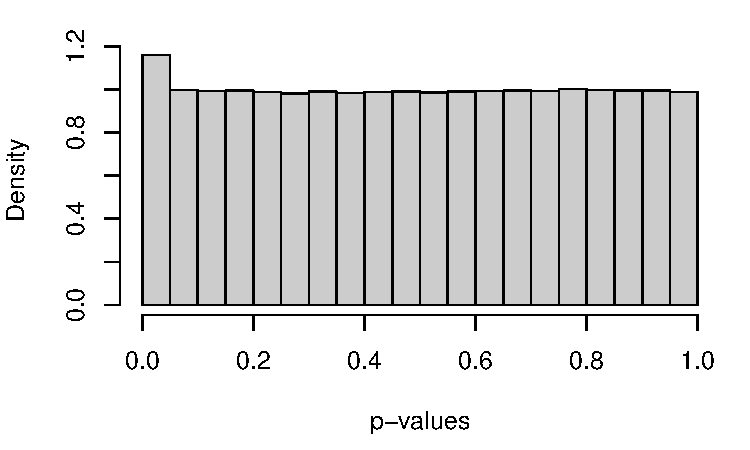
\includegraphics[width=4in]{../graphs/lipidspval}

\vskip .2cm

The tiny spike down by zero is our only hope for discovery.

{\gr Recall: p-values from the null distribution are uniform.}

\vskip -.5cm
\end{frame}

\begin{frame}
{Controlling the False Discovery Rate} 


\vskip .15cm{\sg
The slope of the FDR-cut line is { q/[{\scriptsize{\tt \#}} of variables]}.
}

\vskip .15cm
\hskip .5in
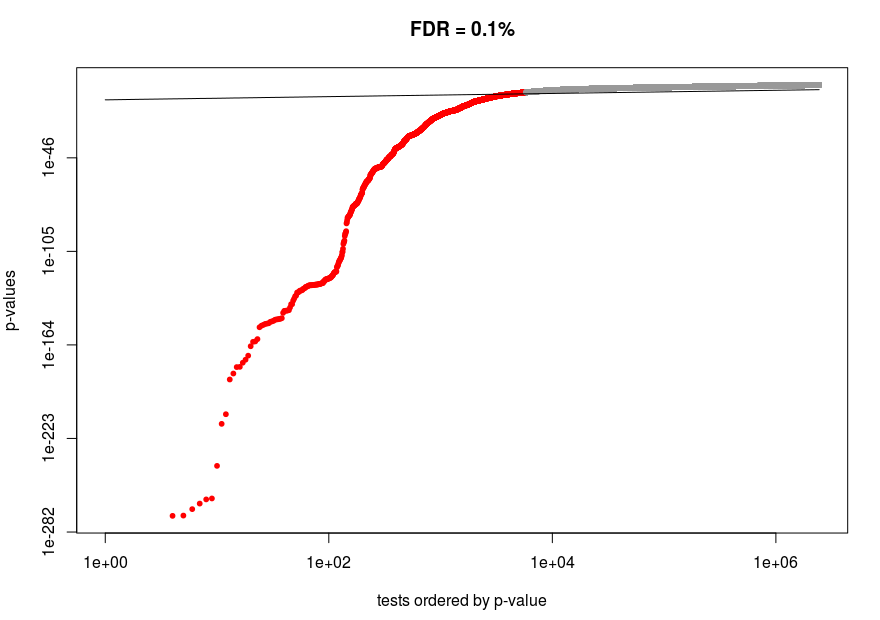
\includegraphics[width=3in]{../graphs/lipidsfdr}

\vskip -.2cm
{\scriptsize \hfill {\color{red}$\bullet$} ~  significant ~~~ {\color{Grey}$\bullet$} ~ not significant}~~~~~~~~~~

\vskip -.1cm
{\theme Lots of action!} \\
4000 significant tests at FDR of {\tt 1e-3} \\( so only 4-5 are false discoveries ).

\vskip -.2cm

\end{frame}


\begin{frame}
{All there is to know about FDR}


p-values from the null distribution are uniform, and 
$N$ of them ranked and plotted should lie along a line with slope $1/N$.
\vskip .3cm
FDP is the number of false discoveries divided by the number of test results called significant.
You don't know the FDP.
\vskip .3cm
You can control $FDR = \ds{E}[FDP]$ to be $\leq q$ amongst $N$ tests
\begin{itemize}
\item rank and plot p-values against rank/$N$
\item draw a line with slope $q/N$
\item find the max point where p-values cross this line, \\
  and use that point to set your rejection region.
 \end{itemize} 

\end{frame}


\begin{frame}
{R roundup}

{Quitting R: usually save the script, not the
  workspace.}\\
{\gr The workspace is an  {\theme .rda} image, while  the {\theme .R}  script
  is just text.}\\

\sk
{\nv Stay up-to-date: \bk Make sure you have latest versions.}

{\nv Stay organized: \bk keep track of your work. }

{\theme Keep things simple, and don't panic.}

\sk Consider using shared drives to collaborate.  Or, even better,
create a group github repo and use version control.

\sk
{R is a  fantastic tool and there is tons you can
  do,  but don't worry about learning everything right away. }

\vskip .25cm
Plenty of resources out there.  Also don't hesitate to use me and your friends (and google!) to avoid frustration.
\end{frame}

\begin{frame}
{Week 1 Homework}

\begin{columns}[c] 
\column{1.9in} 

\sk
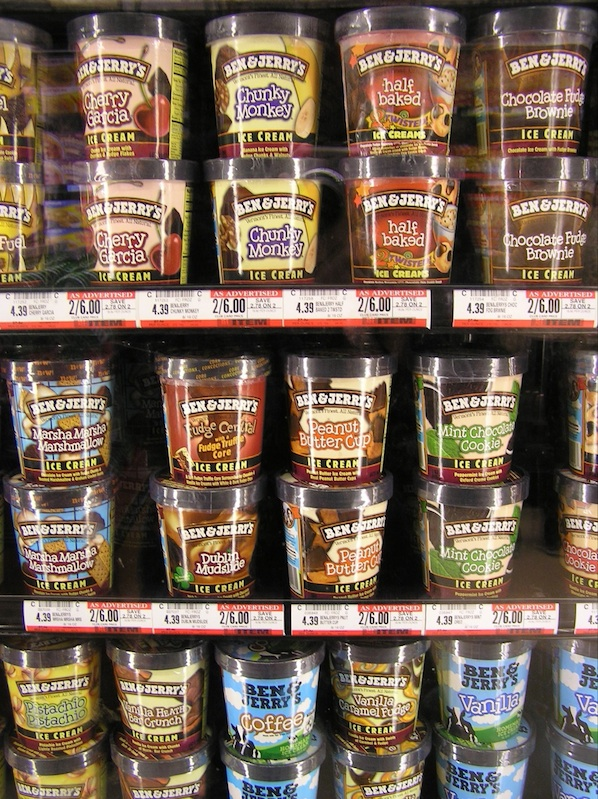
\includegraphics[width=1.9in]{../graphs/benjerShelvesSmall}
\column{2.1in}

{\bf 
Homescan data from Nielson}

\vskip .25cm
70K Households\\and {\theme all} of their purchases.

\vskip .25cm
{Homescan data dictionary\\ is on the course site.}


\sk
\theme Ben and Jerry's \bk subset is in \\~~~{\large\tt BenAndJerry.csv}



\end{columns} 

\end{frame}


\begin{frame}
{Week 1 Homework}

See {\tt benjerry\_start.R} for code to get you started.

\vskip .25cm
[1] Explore the data and visualize:  what variables are interesting?  Choose a few, plot them together, and tell a story.

\vskip .25cm
[2] Describe the regression model in the code.  Improve it?

\vskip .25cm
[3] Take the p-values from your regression and look for evidence of association.
Relate what you learn to your story from [1].  How many true discoveries do you think we have?

\vskip .25cm
[+] Why should we be worried about our FDR control here?

\sk
You are encouraged to work in groups of up to 4.\\   
{\gr Tell me what you find (and how). \gr Do not hand in R-code!}\\
Homeworks are out of 5: {\sg Amazing, Great, Good, Poor, Ouch. }

\end{frame}

\end{document}
